\chapter{ROAR}
\label{ch:roar}

% pull some sort of epigraph from mcluhan? not sure exactly what it would be, but something about TV audiences.

The projects described thus far: \emph{Information Spaces}, \emph{Presentation Spaces}, \emph{backchan.nl}, and \emph{Tin Can} are all interested in supporting audiences who are not merely passive receivers of information, but active participants in an experience. My interest in non-verbal actions as a design technique is the main way I accomplish this. This is an important and effective strategy because verbal participation becomes more challenging as the number of potential participants grows. As discussed in Chapter \ref{ch:intro}, the constraint that only one person can talk at a time and the switching costs with synchronous verbal communication impose stiff costs on the engagement level of a group as that group size increases. I have sought in my designs to alleviate these costs by creating other ways to participate that don't have the constraint of seriality, which in turn frees us from the costs of negotiating turn-taking. I have shown the various ways this can create experiences where people feel more engaged with the process, more connected to the audience, and feel like they have an impact on group process in ways that traditional ``being there'' approaches to mediated interaction have trouble providing.


Still, these approaches have limits. As audiences scale up beyond a few hundred (in the case of the largest \emph{backchan.nl} events we've observed), the design approaches we've proposed start to break down.\sidenote{This is not specific to mediated interactions; interactions between unmediated communities change dramatically as the size of the community goes up, too. \citep{dunbar_number}} With \emph{backchan.nl} specifically, the first failure mode is that the ``recent'' posts section becomes overwhelmed and hard to keep track of. This causes many users to simply opt out of voting on new posts because they appear faster than they can practically judge them. Larger audiences also bring increased odds of abusive behavior like spamming and mass-voting for low-quality posts. One common approach to handling increasingly large groups is to segment them into manageable chunks where our traditional techniques work well. \sidenote{Often this segmentation happens for technical reasons as much as social reasons. Maintaining a sense of presence in a mediated group tends to be an $N^2$ scaling problem. The scaling factor is particularly brutal for virtual worlds which tend to have problems even rendering large numbers of avatars, let alone managing the communication problems of letting them interact. This has let many systems simply avoid the problems of large scale interaction because they were technically unrealistic.} This works, but it's a bit of a dodge. This chapter will argue that there are ways to simultaneously create compelling small-scale experiences that provide synchronous text-based interaction (e.g. chat) while also providing a series of mechanisms that help a very large group stay aware of each other's moods and interests and engage in various forms of collective activity that make it feel like you're really part of a very large audience. Thinking about mediated crowds in this way brings up compelling conceptual questions like: 

\begin{enumerate}
\item{How do people find groups of people to talk with?}
\item{Do collective activities like chanting or doing the wave have online crowd analogs?}
\item{How do you manage antisocial behavior in online crowds?}
\item{How can you create opportunities for deeper engagement with the event that have an impact on other audience members' experiences?}
\end{enumerate}

Constructing a sense of remote viewership is not a new activity. As radio, film, and television broke down removed the physical constraints of audiences and performers being co-located, we were able to create enormous audiences all experiencing something together. Yet there was clearly something important about the presence of the audience. We still go to movie theaters to watch movies together, and TV shows frequently have live audiences (or simulate live audiences with a laugh track) to try to foster a sense of experiencing something with someone else.

Over time, the structure of these events has even evolved to take advantage of technology to create a sense of engagement and involvement. Shows like \emph{American Idol} use text messages to allow audiences to vote for specific contestants. This is a relatively thin form of engagement: feedback is quite delayed, votes are essentially anonymous, and the pool of votes is huge which makes it hard to feel like you're making a difference. Nevertheless, this is part of a long-term campaign on the part of broadcasters to try to make it fee like broadcast television isn't simply receiving data, but trying to bring back the historical experience of being in a crowd with other viewers.

In this chapter, I will describe a system called \emph{ROAR} that tries to develop the design techniques described and studied in past chapters towards audiences of extremely large scale. I will talk about related work in the social TV space as well as discuss the other sorts of tools that people use to create similar sorts of experiences. Finally I will describe the major components of ROAR's design: sections, pulse, shouts, and feedback. 

Unlike the main projects in this thesis, \emph{backchan.nl} and \emph{Tin Can}, I have not done any deployments of \emph{ROAR}. This is primarily for practical reasons. It is quite difficult to reach audiences of the sizes for which \emph{ROAR}'s design is specialized. Organizations with audiences of this size tend not to be interested in trying prototype code during a large scale event. Still, these sorts of explorations can provide valuable guidance about a design space that we might otherwise overlook because it is prohibitively difficult to deploy prototype code. As a capstone to a series of more elaborately studied systems, I view this chapter as a forward-looking description of future work that can show how the principles developed in earlier chapters could grow to address the needs and interests of larger public audiences.

With this shift towards larger and public audiences, I've also chosen to design for more practical technical infrastructures. Unlike with virtual worlds in Chapter \ref{ch:virtual}, extra projectors and screens in Chapter \ref{ch:backchannl}, or per-person tablets in Chapter \ref{ch:tincan}, the systems described in this chapter don't expect elaborate pre-existing technical infrastructure and are instead designed to work with whatever platforms already have available. Practically, this means designing for desktop web browsers, mobile phone browsers, and tablet browsers. This also entails a movement away from more speculative design approaches that expect significant changes in behavior to designs that instead aim to emulate and extend existing practices in less radical ways. 


% talk a little more about that, re: tablets and phones as alternate platforms, heweing more closely to existing practice, etc. 








% on co-located audiences, broadcasters discovered the challenges of 
% 
% made it technically possible to assemble remote audiences, we were left 
% 
% 
% The transition from co-located audience to remote audience was an uncomfortable one. As audiences 
% 
% Broadcast media like radio and television created the modern audience. More than any of the other technologies described in this thesis, only broadcast media have created truly enormous simultaneous audiences. Broadcasting live events broke down the physical constraints involved in creating a space that could support large local audiences. It became possible to share at least a portion of the experience of watching something live while being at a distance. 

% talk about how spaces evolved to support the remote audience. cameras as the eyes of the masses. remove viewers giving experience meaning. shift to small ``studio'' audiences. the laughtrack and roar of the crowd to give meaning to the remote experience. simulating an audience.

% trace history of how events evolved to become better aware of the remote audience? incresed value of space in the remote visual field (e.g. advertising that shows on screen only, not in the physical space - provides local addressing). 



% topics in a random order (for now)
% scaling non-verbal actions (distribution approaches, viral spread mechanics, etc)
% creating small scale interactive groups
% 	can put the twitter arguments here - why having bounded audiences is good + how to discover those audiences
% synthesizing interaction
% 	talk about the chat visualization systems.
% 
% how to organize this chapter?
% 	one model is to march through a series of designs and talk about the evolution. In this model we would do:
%	original trending words view
%	first prototype
%	second prototype visualizations
%	final version
%
% the challenge is a lot of the pieces are more conceptual and don't necessarily "exist" in any of these prototypes. shouts and questions and votes and betting are all good examples of that. this is an argument for laying out the basic strategies in a conceptual way and then moving through the concrete prototypes with those in mind. Treat the prototypes as instantiations of those visions and just say "oh, this is what changed". 

% so final strategy is:
%	introduce the field
%	talk about the history of audiences (maybe, this isn't my strong point)
%	talk related work (put the why not twitter, why not facebook section here)
%	set out the values here
%	series of modular approaches: sections, pulse, shout, voting/betting, 
%   future directions (representations in the physical arena, creating new streams of content, tumblr-like engagement, etc)


\section{Related Work}

% really need to do at least a cursory walk through the CHI/CSCW literature on social tv stuff. I know frank did stuff like this back in the day.
%
% A Visual Backchannel for Large-Scale Events
% get andrea's bibliography and pull from there

\subsection{Alternatives}

There is a widely-held assumption that interaction around live events like those that \emph{ROAR} aims to support are already taking place on existing social networks like \emph{Facebook} and \emph{Twitter}. If this were true, it would suggest a very different approach; one that looks much more like \emph{Visual Backchannel}. However, I will argue in this section that the social spaces created by \emph{Facebook} and \emph{Twitter} are not (and barring pretty fundamental changes to their mechanics can not become) spaces for truly interactive discussions about a live event.

As I've argued about grounding elsewhere in this thesis, creating social situations with mutual awareness is critical to creating effective conversation spaces. If there is any concern that others can't see what you're saying, it breaks the cycle of awareness that is critical for moving a conversation forward. The publish/subscribe model adopted by and \emph{Twitter} gets in the way of this once conversations scale beyond just one person. If Bob follows Alice, and Charlie follows Alice but not Bob, Charlie will see only parts of a conversation that are not directed at Bob with an ``@'' reply. \sidenote{I'm going to mostly ignore \emph{Facebook} for the sake of simplifying the argument. The outlines of the argument are similar, but \emph{Facebook}'s more integrated reply format avoids some of these problems. But the lack of reliability of posts being seen by followers (as few as 20\% of your followers see any given post \citep{facebook_post_seen_freq}) adds another challenge to creating a grounded community.}

The nominal solution for this is hashtags, e.g. words prefixed with a ``\#'' character. These mark a tweet as part of a larger set of tweets on a theme, and places that tweet in a stream in the so-called ``discover'' part of the interface. This interface has a similar grounding-inhibiting design. First, it is impossible to tell if others are actively viewing the hashtag in the ``discover'' mode. Whether or not that audience exists is essentially unknowable to posters. Hashtags are visible amongst follower networks (i.e. you can see hashtags that seem to be popular within your network and be involved in this conversations) but there is little evidence that participations cross existing follower/following relationships.

The problem of an audience for tweets with a hashtag is compounded because tweets with a hashtag do have one guaranteed audience: your existing followers. Every tweet, hashtagged or not, is inserted in the streams of all your followers. When balancing a potential imagined audience and a guaranteed one, people will write for the audience they know they have. For major events like the Superbowl or World Cup, we can safely assume that our audience is likely to contain many people who are watching the same event. But even for moderately less popular events, it is far more likely that most of our followers are not co-watching and are unlikely to be deeply interested in a detailed conversation about what's happening. 

We can see that this is true by looking at the sorts of tweets that people write during live events like conferences. \citet{Ebner:2010tx} try to categorize conference tweets into four categories: irrelevant tweets, administrative tweets, topical discussions, and topical tweets. The distinction between the latter two categories seems to be whether a tweet contains an ``@'' reply or not. The authors argue that without external information like a link or picture, a tweet is too decontextualized to be valuable to a non-attendee. I see their data differently. If we look at their exemplar topical tweets (excluding questions, whose audience is clearly the presenter), most of them are clearly written for an audience that does \emph{not} share their context.  For example, the tweet ``nice idea of @estudyskills Aggregation of all student weblogs at Tumblelog - gives overview. \#ec10hh'' is recording the content of a talk for someone who isn't there. A simple evaluation-oriented tweet like this for a co-present audience would look a lot more like ``nice idea of @estudyskills'' and leave off the rest of the context. Indeed, this is the core difference between chat messages and posts to \emph{Twitter} or \emph{Facebook}: chat messages rarely make sense out of context, but posts are nearly always written with context included to make them comprehensible to a non-present audience. 

% do an informal analysis of tweets for the latest ML talks event. categorize into announcements, quotes, other https://twitter.com/#!/search/realtime/mltalks

While looking at how people write tweets versus chat messages is interesting, volume of participation is also interesting. We can look at summary data from Bluefin Labs, a company that captures and analyzes \emph{Twitter} conversations about TV shows and compare the participation rates in \emph{Twitter} conversations to similar chat conversations. For each show they analyze, they report the total number of tweets about the show and the total number of people who tweeted about the show. The ratio of these two values is the average number of tweets per tweeter. For the vast majority of shows they track, this value is between $1$ and $2$; the average viewer tweets at most twice about a single show. This holds true even for sports matches that can last 2-3 hours. It is intuitive that only one or two messages per person is a strong indication that there is not significant conversation going on; conversations simply cannot take place in one or two messages. Nevertheless, it is useful to compare these participation patterns with a social context that looks more like \emph{ROAR} to argue for \emph{ROAR}'s design approach.

% put in a screenshot of the blue fin data page

Although we don't have data for people using a system like \emph{ROAR} yet, we can look to comparable experiences that already exist. Many sports fans use platforms like Internet Relay Chat to talk about live events. Based on logs collected over the course of two weeks, we can calculate a metric similar to that reported by Bluefin Labs for conversations on \emph{Twitter}. We can't easily link specific messages to specific events, but we can measure how many messages each person sends per hour in which they send any messages at all; essentially for people who are chatting in a given window, how many messages do they send? This approximates the tweets per unique author per show metric. This measure varies pretty substantially between which chat room you collect data from. Data is reported in Table \ref{tab:chat_message_rates}. 


% channel name
% average unique hourly users (average )
% total messages  \sigma{msg}
% total duration t_n - t_0
% average messages per active user
% comments

\begin{table*}[tb]
\begin{tabular}{r|lllll}
\textbf{Channel} & \textbf{Total Messages} & \textbf{Total Users} & \textbf{Mean Hourly Active Users} & \textbf{Mean  Messages Per Active User-Hour} \\

\#reddit-soccer & 20,317 & 251 & 7.9 (SD=9.9) & 16.6 (SD=25.5) \\
\#football & 11,936 & 199 & 8.8 (SD=8.2) & 10.1 (SD=11.8) \\
\#teamliquid & 110,910 & 1,940 & 29.7 (SD=19.2) & 9.5 (SD=18.1) \\
\#joindota & 93,010 & 9,022 & 52.8 (SD=113.3) & 3.4 (SD=9.6) \\
	
\end{tabular}
\label{tab:chat_message_rates}
\caption{Comparison of participation rates across different IRC chat rooms.}
\end{table*}

The most direct comparison to \emph{Twitter} is the final numeric column on the right. Mean messages per active user-hour represents the average number of chat message a user sends in hours where they send any messages at all. If every user logged on, sent one message, and then stayed silent, this metric would be 1. It would also be 1 if every user sent one message per hour. As a result, the floor of this metric (as with the tweets / unique author metric) is 1. Larger values represent users who tends to send many more messages during hours where they are chatting at all. This metric is artificially depressed relative to the \emph{Twitter} metric because our data covers not just moments when there are live events going on, but 24 hours a day. This is captured by the variance in the fifth column: the number of active chatters varies widely between active moments and inactive moments. Inactive moments don't exist in the \emph{Twitter} dataset because it focuses on only the tweets associated with a television show. Despite this, we see values ranging from 3.4 to 16.6, compared to \emph{Twitter}'s 1-2. This suggests that chat contexts elicit a 200-1600\% increase in per-active-user participation. 

The large variance in participation rates seems (in this very preliminary review) to be correlated with the size of the rooms. The rooms with the highest per-user participation were also the rooms with the fewest active users. This supports the \emph{ROAR}'s core argument that smaller interaction contexts will be more interactive than larger undifferentiated contexts. This might also explain part of the difference between \emph{Twitter} and a chat-style system: \emph{Twitter} looks much more like a single large undifferentiated room than a focused small scale social space.

This informal analysis underlines both the strong differences in behavior in post/subscribe models like \emph{Twitter} or \emph{Facebook} compared to chat-based designs like \emph{ROAR}.




% We can see th

%The easiest way to understand that is does is exist would be getting a reply from someone who doesn't follow you who discovered your tweet via the ``discover'' tab. Although this is possible, a casual perusal of tweets involved in trending topics shows vanishingly few replies to other tweets; RTs are far more common. These impediments to mutual visibility 

% would be interesting to make an empirical argument about how many @ replies are to people via hash tags. could try to do this by looking at @ that were replied to that were between people who don't follow each other and have used a hash tag in a period. that's a bit elaborate, though. 

% make a diagram of the alice/bob/charlie system
% put a screenshot of the discover interface in here in



\section{Design}

\emph{ROAR} is a social platform that wraps streaming video of a live event. This section will cover the basic components of a web-based version of \emph{ROAR}. An overview of the visual layout is shown in Figure \ref{fig:roar_overview}. 

\begin{figure*}
	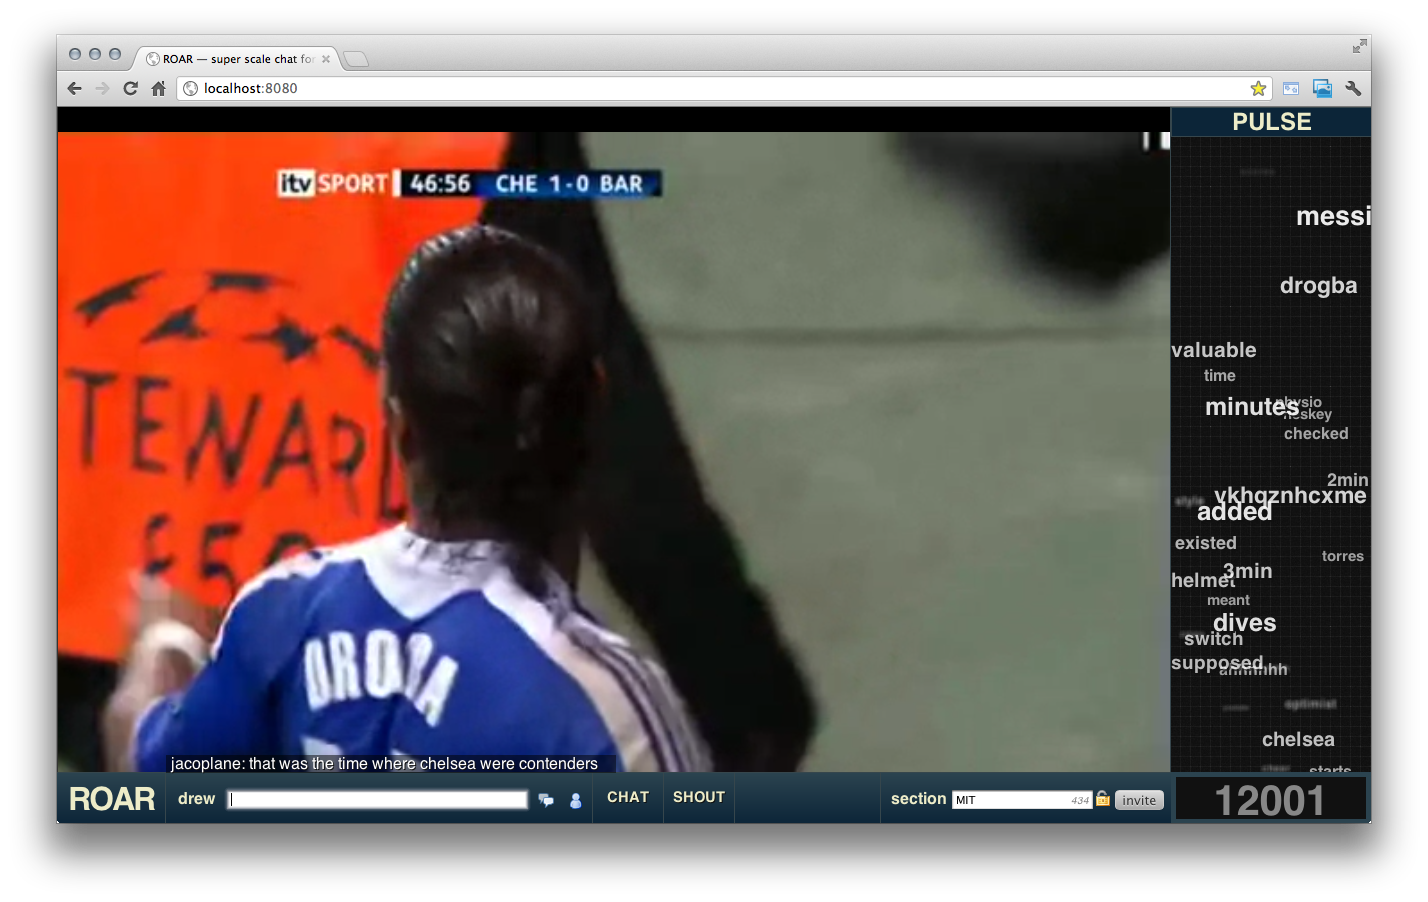
\includegraphics{figures/roar/overview.png}
	\caption{An overview of the \emph{ROAR} interface.}
	\label{fig:roar_overview}
\end{figure*}


\subsection{Sections}

I take the organizing metaphor of a ``section'' from the physical experience of being in a crowd at, for instance, a sporting arena. Audience members rarely come to a stadium alone: most people come with friends. Existing tools for watching live events with chat tend to simply group all viewers into one anonymous mass. As I argued in the previous section, this approach tends to depress overall participation because too much chat can crowd out deeper and broader conversations. In contrast, \emph{ROAR} organizes viewers into many  smaller sections. Each section can be named or unnamed. 

When a viewer joins a \emph{ROAR}-enabled stream, they are provided with a section browser. If they log in with a \emph{Facebook} or \emph{Twitter} account, \emph{ROAR} can prioritize sections with friends in them. A draft of this interface is shown in Figure \ref{fig:roar_section_browser}. For viewers who don't want to log in with \emph{Facebook} or \emph{Twitter}, they can search for named rooms on a particular theme, like a school, employer, location, or team they're a fan of. Conceptually, sections are like tables at a bar or circles of people at a cocktail party. You're likely to know at least some of the people at a table you want to join, but not necessarily everyone. It's easy to scan the room to evaluate options. When you're in a section, most of your attention is focused on the interaction within that section, but there are a number of other systems that try to maintain some awareness of the crowd as a whole. 

\begin{marginfigure}
	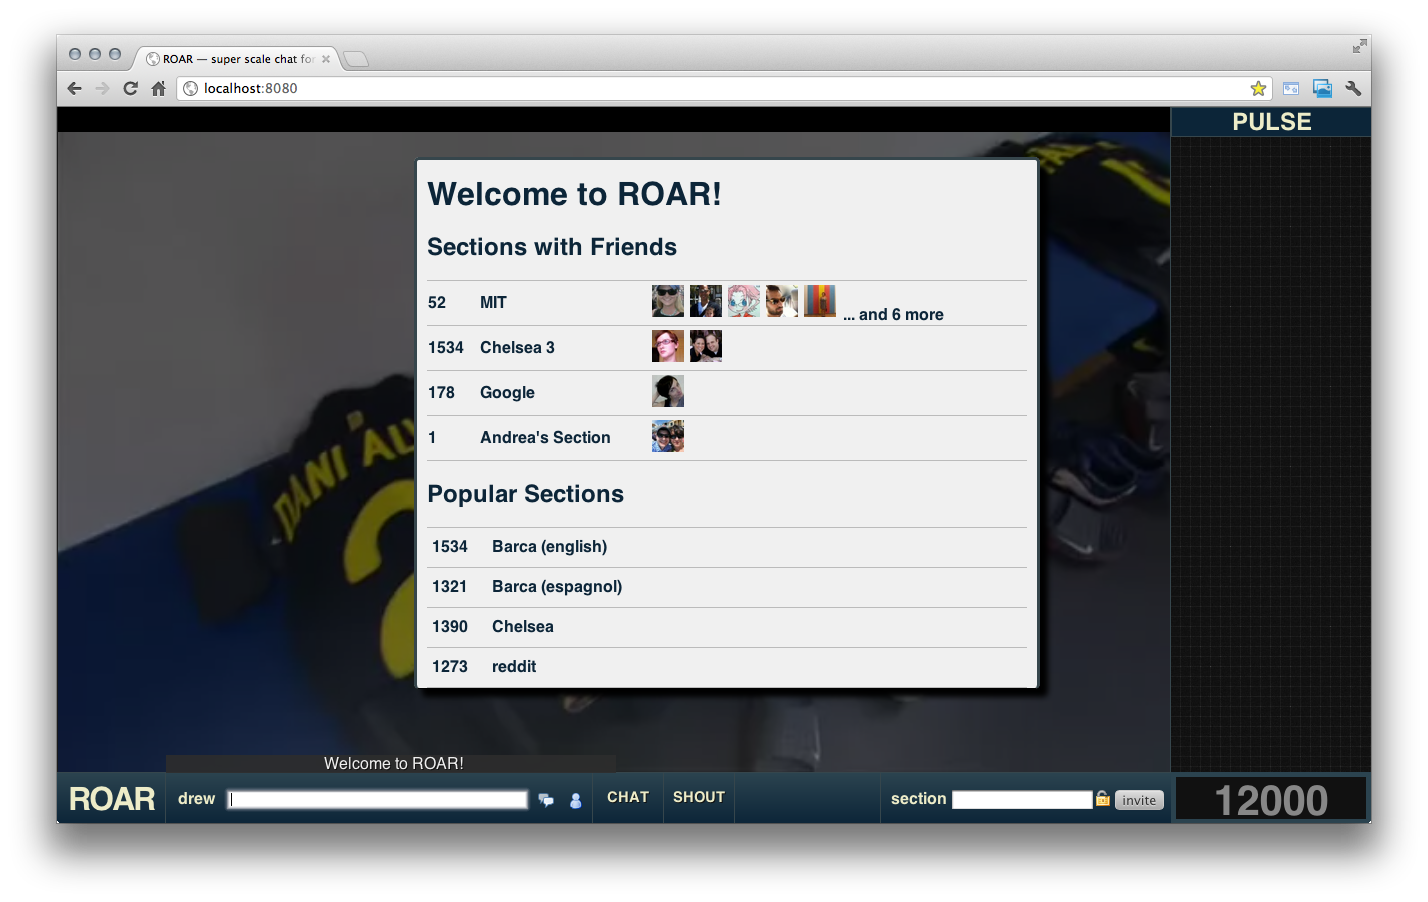
\includegraphics{figures/roar/roar_sections.png}
	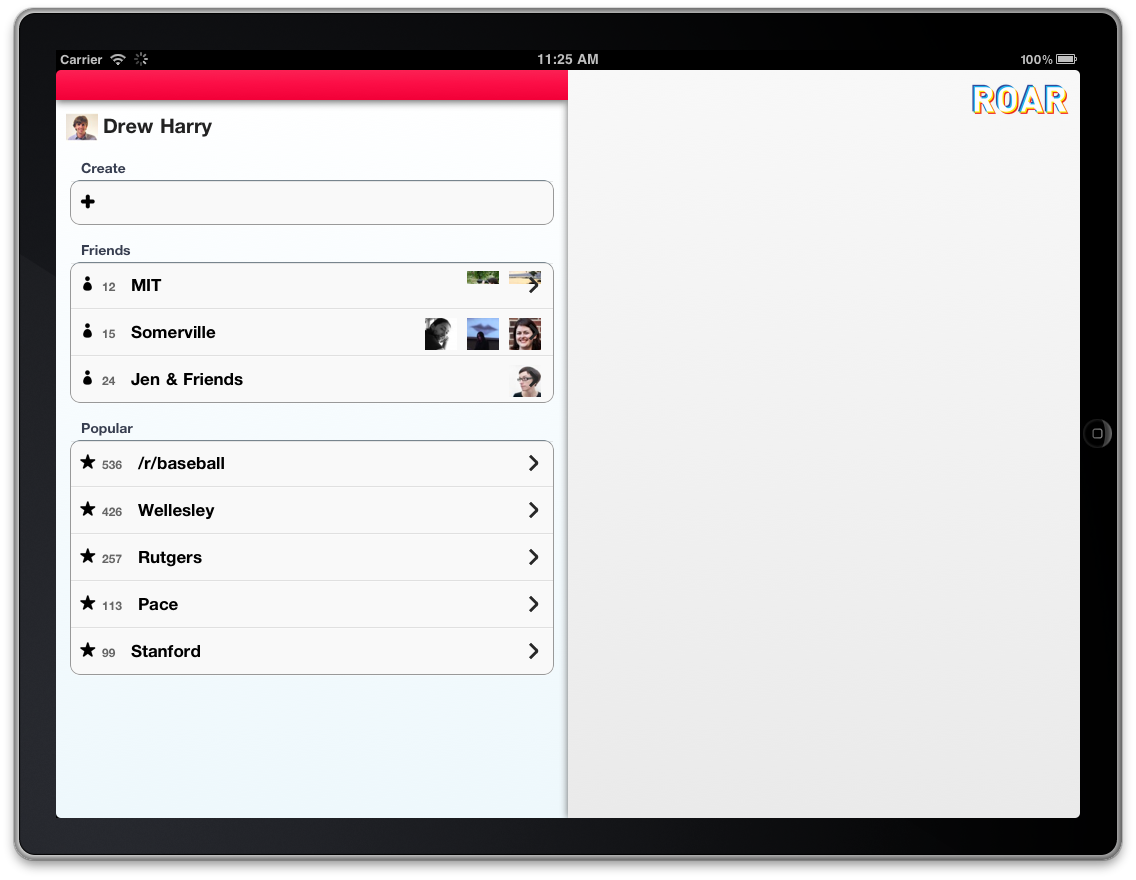
\includegraphics{figures/roar/roar_sections_tablet.png}
	\caption{View of the section selection interface on a web interface (top) and tablet interface (bottom).}
	\label{fig:roar_section_browser}
\end{marginfigure}

There are a variety of potential interaction styles within a section. Chat is the dominant one shown in this prototype, but chat depends on easy access to a keyboard. It is easy to imagine versions of \emph{ROAR} that would make sense on a mobile phone or tablet device. In these contexts, text entry is somewhat more challenging, so having interaction models that require less text entry but that still support a sense of presence would be valuable.

There are two varieties of interaction that the \emph{ROAR} prototype supports. The first is the ``shout.'' Shouts are composed less like chat messages, and more like tweets. They are intended to be shared out of context to more people. A shout might be a witty comment, a link to a funny image about the game, a clever insult to a hated player or team, or simply a message that captures the feeling of the crowd at that moment. When a shout is entered, it is shown first to viewers in the section of the author. Unlike chat messages, shouts can be voted for. Shouts that accumulate enough votes within their initial section will spread to other sections. \sidenote{There are a number of moderation challenges with shouts that will be addressed later. Shouts are also significantly rate-limited, and having previous shouts judged negatively by a moderator will strongly increase this rate-limit.} Eventually, widely popular shouts could spread to the entire audience, while some will peter out having only been seen by a small fraction of the crowd as a whole.

The second variety of novel interaction is the creation of graphical signs. Although this doesn't make much sense with a traditional keyboard and mouse interface, drawing is much more natural on tablet devices. For users in that context, drawing can be more expressive than typing. The creation of signs meshes nicely with existing fan practices around bringing signs to a stadium. Indeed, signs brought to the stadium are explicitly written to attract the attention of camera-operators and commentators with the hope of being broadcast to the remote audience and put on a live display within the stadium. In this way, the practice of sign creation is already implicitly acknowledging the attention and awareness of the remote audience. Empowering remote fans to participate in this practice seems like a natural extension, especially on input devices where drawing is easy and accessible. An example of the drawing interface and a sign's representation in the section stream are shown in Figures \ref{fig:roar_sign}.

\begin{marginfigure}
	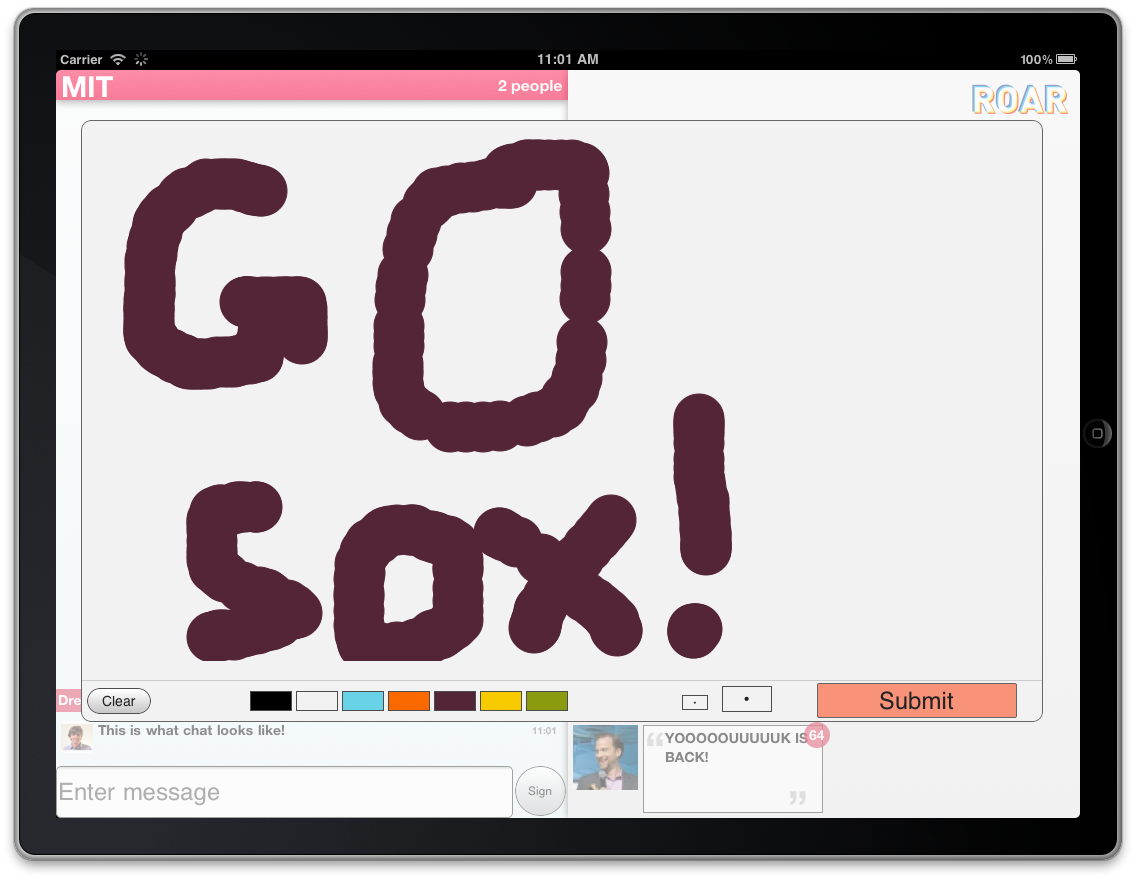
\includegraphics{figures/roar/drawing_sign}
	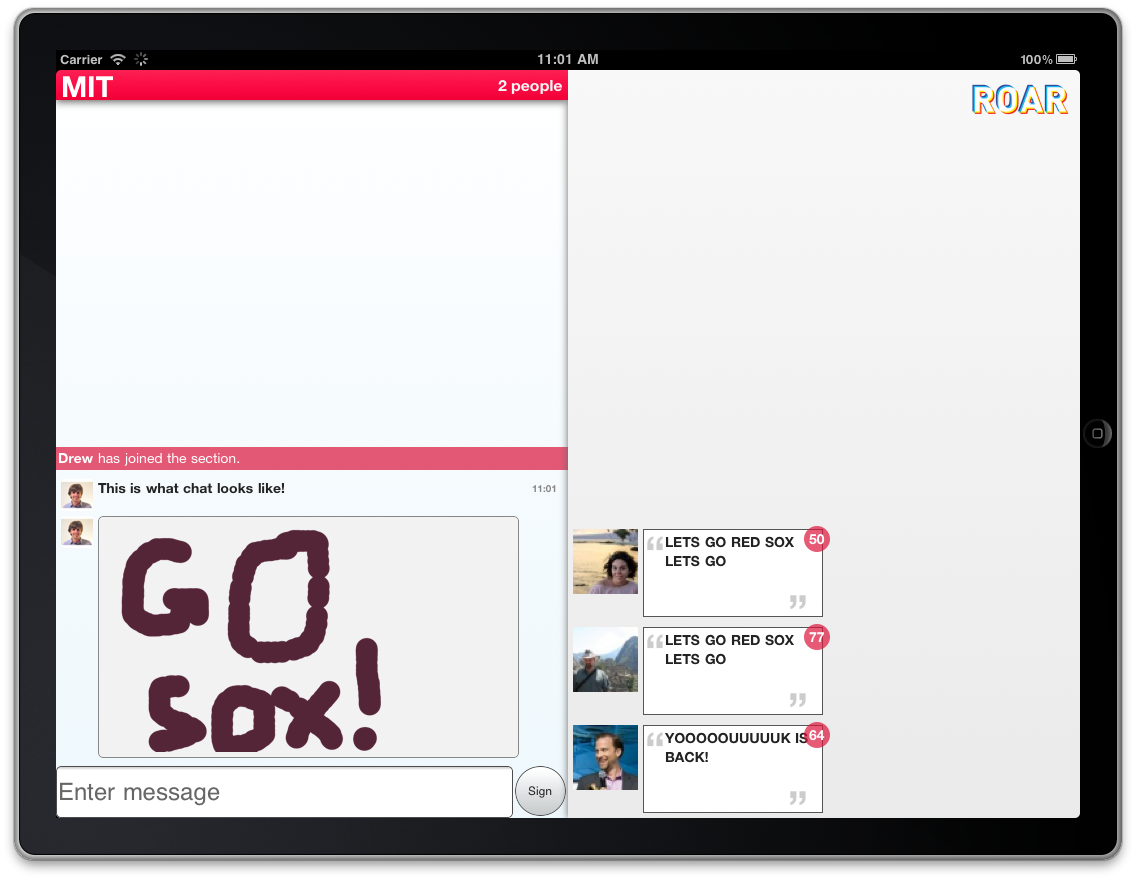
\includegraphics{figures/roar/sign_in_section_chat.png}
	\caption{Top, an interface for drawing a sign in a tablet interface. Bottom, that sign displayed in a section stream.}
	\label{fig:roar_sign}
\end{marginfigure}

% talk about question-asking ala backchannl? probably not.

As a primary communication medium, non-audio communication has a number of major advantages for \emph{ROAR}. Chat requires minimal extra hardware, can be done in loud places, is more easily analyzable at large scales, doesn't require turn-taking, and requires substantially less technical infrastructure to support at scale. Still, it is far less immersive and communicative than voice communication. Although audio becomes problematic for large groups (for reasons discussed throughout this thesis), the potentially small size of sections might mean that for groups of 3-5 audio could be an effective addition.

% TODO talk about section categorization and recommendation? 


\subsection{Predictions, Betting, and Promoting}

Although chat is the foundation of creating a sense of presence with other people in a section, this thesis has argued throughout for the value of non-verbal actions that provide lighter-weight senses of presence. These kinds of actions can help remind section-members of the presence and engagement of people who might not have something to say, but are still attending to the section and the event. In the context of \emph{ROAR} there are a number of different kinds of non-verbal actions that would be appropriate.

The most simple of these actions is making predictions. An event organizer could pose a question to an audience like ``Which team will win the game?'' These questions could be section-specific or global. Responses to a prompt like this can be aggregated globally or (more importantly) be represented within the section to catalyze a discussion. A simple version of this is shown in Figure \ref{fig:roar_voting}. These questions could also come from section-members and be scoped just to the section.

\begin{marginfigure}
	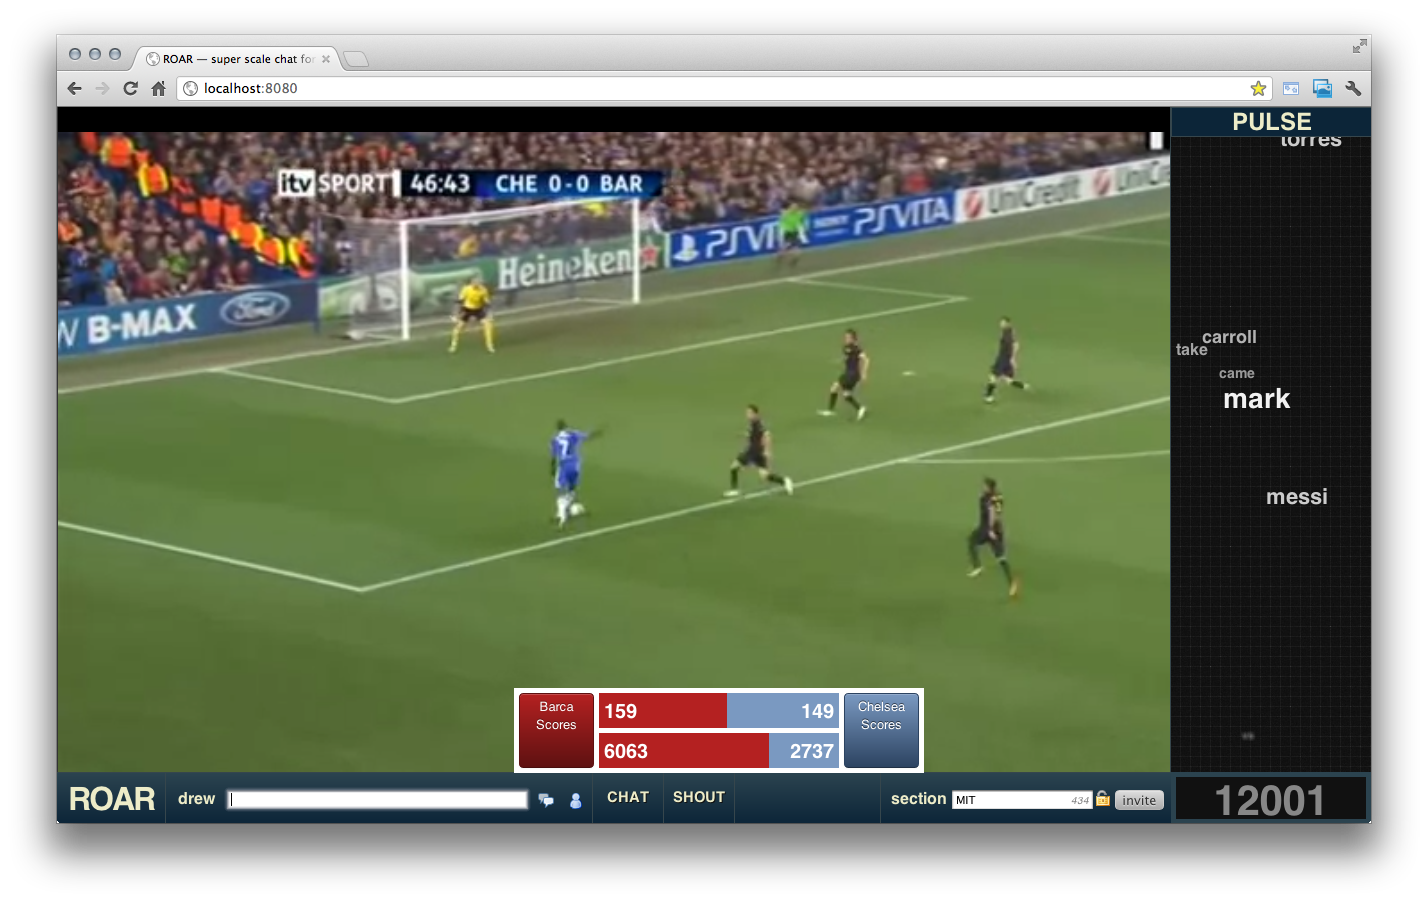
\includegraphics{figures/roar/voting.png}
	\caption{In the bottom center of the screen, an open vote. The top bar is votes within your section, the bottom bar is global votes.}
	\label{fig:roar_voting}
\end{marginfigure}

These sorts of lightweight predictions make sense across a wide range of the sorts of events that \emph{ROAR} aims to support. Live competitive performance shows like \emph{American Idol} or \emph{The Voice} have occasional moments where the audience could weigh in and change the course of the show. Sports-oriented events could offer an even more elaborate and high-frequency interaction. Instead of the occasional audience-wide poll, fans could place time-sensitive bets on the outcomes of various game events. Baseball provides a particularly effective example. Within a single game, there are a series of interlocking time scales where predictions make sense from the inning to the individual batter, to the individual play. At each of these levels, a viewer could opt to place a bet about the outcome of the event. These bets would be shared at the section level, and effective betters would be highlighted on a leader-board. While these kinds of actions don't make sense for all events, they're another design element that could be added or subtracted depending on the style of event. 

All sorts of section and crowd-level participation can also support voting to guide the promotion of interesting content and the identification of inappropriate content. This serves as an additional stream of non-verbal actions for the engaged but perhaps not verbally inclined viewer. Votes are aggregated for shouts and signs, and used to spread those contributions to a wider audience. This serves to create a stronger relationship within the audience. By participating in identifying the sorts of content you like, it creates a sense of the community's values represented in the top contributions as judged by viewers. It also supports a sense of ownership. Without voting, the acknowledgement of a crowd contribution on-air (in the way that cable news now frequently takes tweets out of context and discusses them on-camera) seems arbitrary and analogous to shouting requests to a band during the breaks between songs. Whether a message catches the attention of the performer or anchor is essentially arbitrary. But by being able to identify contributions that you see as valuable, you can buy into the success and quality of that contribution and celebrate its broader spread rather than rue the arbitrariness of a random selection process.

One of the major benefits of nonverbal actions like those discussed in this section is their ease of aggregation. As in \emph{backchan.nl}, where voting serves as a simple low-impact way to participate which guides the system's decisions about what content to show on the main screen, non-verbal actions like making predictions, placing bets, or voting for other kinds of content can be easily aggregated across all sections and represented back to the crowd as a whole. This create a continued reminder of the crowd's presence in the same space. Furthermore, \emph{ROAR} could leverage the existing infrastructure in the physical spaces where events take place to represent the remote audience back to the co-located audience. Using the example of audience-drawn signs, we can imagine using jumbotron in a stadium, for instance, as a venue to share remote audience content that has been voted up. This creates a strong incentive for creating and voting for content because, as in \emph{backchan.nl}, the shared screen carries with it a guaranteed audience for your contribution. Having something you created or promoted appear in the main video stream in a physical space closes the feedback loop, and reminds physical spectators and remote spectators of each others' presence. An example of this approach is shown in Figure \ref{fig:roar_fenway_sign}. As with using shared displays in other projects in this thesis, using existing displays in physical venues can help ground the experience between remote and local audiences and create a stronger sense that they are sharing an experience.

\begin{marginfigure}
	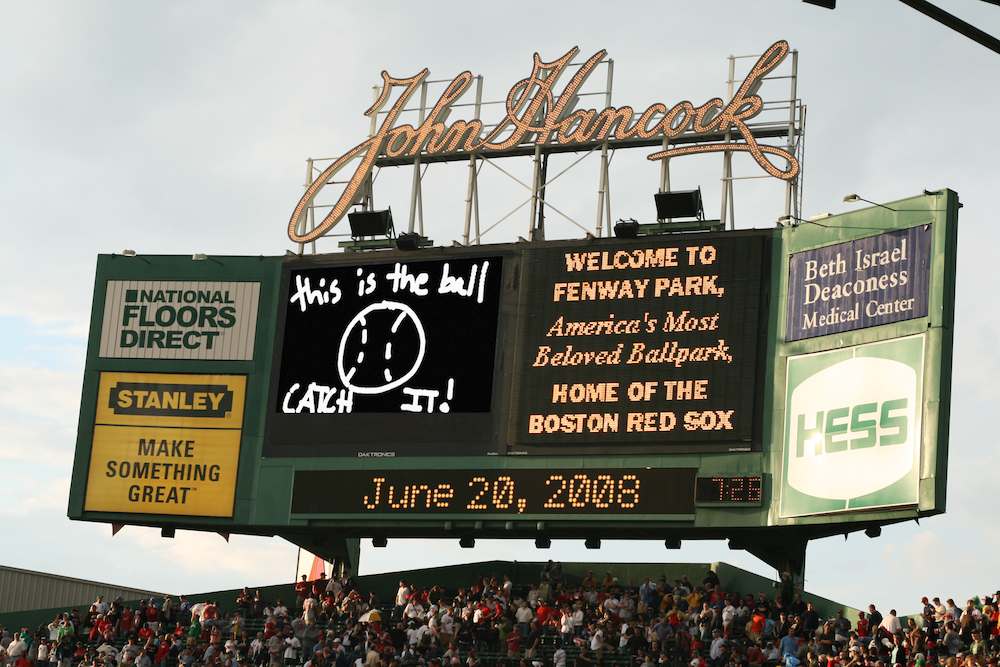
\includegraphics{figures/roar/stadium_sign_small.png}
	\caption{A sign drawn by an audience member displayed on screen in the stadium.}
	\label{fig:roar_fenway_sign}
\end{marginfigure}


\subsection{Pulse}

Section-oriented features focus on creating a small scale sense of community between small groups of viewers. While this is part of an enjoyable spectating experience, an awareness of the crowd as a whole is a critical component to the \emph{ROAR} vision. More than any other feature in \emph{ROAR}, the crowd visualization has evolved considerably over the design process. In this section, I will describe each of these designs, and explore the extent to which they satisfied the different sorts of awarenesses you can have of a physical crowd:

\begin{description}
\item [Volume]{How active is the crowd right now, relative to the recent past?}
\item [Topics]{What topics is the crowd talking about right now, and what are they saying about those topics?}
\item [Collective Action]{More speculatively, might we be able to give the crowd opportunities to do some sort of activity analogous to singing or chanting?}
\end{description}

Each of the designs described here is supported by a keyword detection algorithm that is essentially unchanged across the visualizations. The algorithm scans all chat messages and applies an adapted version of the Term Frequency, Inverse Document Frequency algorithm to identify words that are globally uncommon but frequent in the last few seconds of chat. TF-IDF depends on a notion of documents, and compares the term frequency within a given document to all other documents within the corpus. For a real time stream of data like chat, this obviously requires some adaptation. \emph{ROAR} bins all chat into 10 second windows of chat, and treats those as documents as far as TF-IDF is concerned. This makes sense conceptually because we can assume that chat is about the video, and as the contents of the video shifts over time, the conversation about it will as well. This means we can reasonably assume that each window of chat will function similar to documents in a traditional TF-IDF model. Of course, this assumption is not iron-clad, and can lead to quite noisy results. All the chat shown in screenshots of these visualizations is recorded from Internet Relay Chat rooms organized to discuss various spectator events like video game tournaments or sports matches. 

The analysis engine provides a rank-ordered list on a per-window basis (10s) of the words with the highest recent TF-IDF scores. I call this list the ``term rankings.'' \sidenote{The size of this window is purely a function of chat rate. At high chat rates, this window can shrink substantially and decrease the latency between a new term appearing and it being recognized by the algorithm. At low chat rates, the window needs to grow larger so build larger enough bins to do a reasonable analysis.} This is the input to each of the visualizations described here. It is quite common for subsequent rank ordered lists top words in the last analysis window to share very few words with any previous analysis window. This high amount of turnover poses a design challenge that each design deals with in different ways: how much inertia should be added to the visualization to dampen out the inherent noisiness of the term rankings? 


\begin{figure*}[tb]
	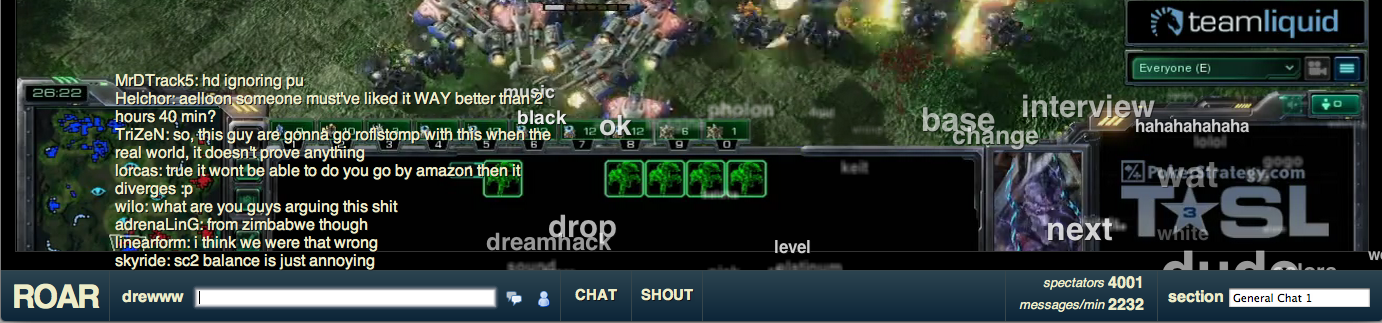
\includegraphics{figures/roar/cloud.png}
	\caption{A word-cloud style visualization where words appear when first seen in a term ranking list and fade over time.}
	\label{fig:pulse_word_cloud}
\end{figure*}

% initial word cloud on top of video

The first visualization adopted a word cloud model. When a word appeared in the term rankings list, that word was added to the word cloud. The higher its position in the term rankings, the larger the initial size of the word. Each second, every word currently displayed in the visualization would decay in size slightly. If a word already displayed in the cloud appeared in a subsequent term ranking list, its size would be increased, correlated with its ranking in the list. If a word slipped below a certain size, it would fade out of the cloud. The cloud was rendered on top of the live video, ostensibly in a part of the screen that was not as critical to viewers. This approach is shown in Figure \ref{fig:pulse_word_cloud}

This visualization had a number of valuable properties in terms of our three original goals. Volume and topics were both easily comprehensible in this format. In particular, the spatial stability of words (i.e. they stay in more or less the same place on the screen for their lifetime) made it easy to both track the performance over time of an individual topic and not be distracted over-much by constant movement. This approach struggled with the temporal component to the data, though. It combines terms that were historically popular but haven't yet decayed enough to be removed with up and coming words. While the lack of a time component simplifies the visualization, it also makes it somewhat less effective for collective actions like cheering or chanting because earlier stages of a cheer are conflated with current ones. Perhaps the biggest problem with this approach is its space inefficiency. Responding to a demo video using this visualization style\sidenote{This visualization can be seen in motion in this demo video: \url{http://www.youtube.com/watch?v=KK13_jE_NGg}}, potential users expressed an intense dislike for any approach that attempted to overlay the video itself. As a result, all future visualizations are located at the edges of the screen using pixels dedicated for visualization, not attempting to overlay the video.

\begin{figure*}[tb]
	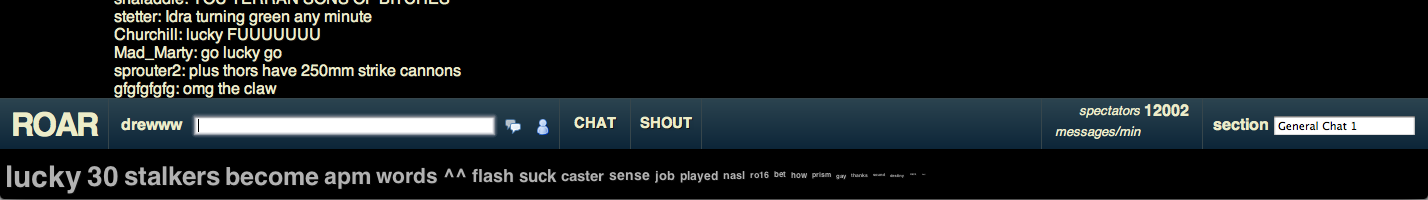
\includegraphics{figures/roar/bar.png}
	\caption{A direct visualization of the term rankings. Larger words have higher rankings, and the total number of words is correlated to the volume rating at that moment. This list changes completely on each new term ranking list.}
	\label{fig:pulse_rankings}
\end{figure*}

The other major drawback of the word cloud approach is the lack of semantics to the position of words. The next three visualizations use screen location in a variety of ways. The most direct approach was to simply display the term rankings along the bottom of the screen underneath the main interface bar, shown in Figure \ref{fig:pulse_rankings}. In high activity periods, words lower down the term rankings were shown. In this way, the total number of words displayed functioned a bit like a volume meter, and the most important words always occupied the same part of the screen. However, the noisiness of the underlying data made updates distracting. A word could easily jump from the top spot to the bottom of the list between subsequent updates, which made it hard to track the life cycle of a term you were tracking. 

Using the same part of the screen, our next approach adopted a river metaphor in which terms would appear on the left edge of the screen when they first appeared in the term rankings and move smoothly to the right. This better introduced a sense of time that was missing from earlier approaches. If words continued to appear in the term rankings, they would grow in size. If they were missing from the term rankings for a few cycles they would fade away completely. This ensured that any word still showing had appeared in term rankings at least once in the last 10 seconds. Furthermore, words that made it all the way to the right edge had at least been present in the term rankings for a while, making the right side of the visualization a reliable space to see long-term popular words. This approach is shown in Figure \ref{fig:pulse_river}.

\begin{figure*}[tb]
	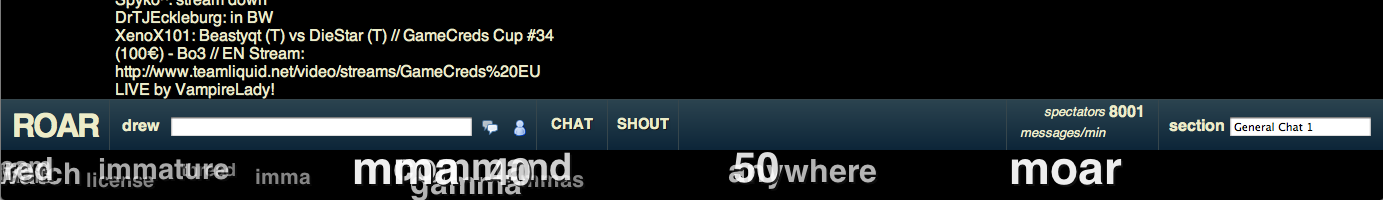
\includegraphics{figures/roar/river.png}
	\caption{In this visualization, words appear on the left edge as they appear in term rankings and move smoothly to the right. Larger words move more slowly than smaller words.}
	\label{fig:pulse_river}
\end{figure*}

While this did create a nice sense of a time passing, there are a number of challenges to this approach. In order to handle a high word density in a tight space, it proved necessary to vary the velocity of each word slightly so they never permanently overlap in a way that makes them illegible. This subtly breaks the contract implied by the spatial configuration; no longer is a word's horizontal position tightly correlated with the age of the term. Furthermore, it seemed sensible for words higher on the term ranking list to be larger, and to maintain a physical metaphor it seemed like larger objects should move more slowly and be on screen longer than small objects. Ultimately, this seemed to be enough at odds with the underlying metaphor that time moves left to right and an object's position on the timeline should represent its age. In a tight visual space, it was too difficult to both satisfy that constraint, make it readable, and manipulate the visibility of words in ways that would properly highlight the highest performing words.

The final design iteration took the basic mechanics from the the horizontal, river-like visualization and mapped it onto the vertical axis. Even with the same basic visualization mechanics, words rising up from the bottom instead of moving left to right helped alleviate the sense that position was mapped tightly onto time. Instead of a river, there is a stronger sense of bubbles rising. To reinforce this sense, a simple visualization of the crowd size could be added in the lower right hand corner, from which the words would appear to be rising. The shifted location within the interface also makes it easier to provide an interactive component. In this version, clicking on a word causes a dialog box to slide into place showing the chat messages that triggered that word's inclusion in the visualization. This provide a convenient way to shift from very high level abstractions on the word level down to individual messages. It might also serve as a way to navigate between sections to spaces where there seem to be interesting conversations happening. This final approach is shown in Figure \ref{fig:pulse_bubble} and Figure \ref{fig:pulse_bubble_detail}.\sidenote{A video version of this approach can be found here: \url{http://www.youtube.com/watch?v=Ky9U1v38zsk}}

\begin{marginfigure}
	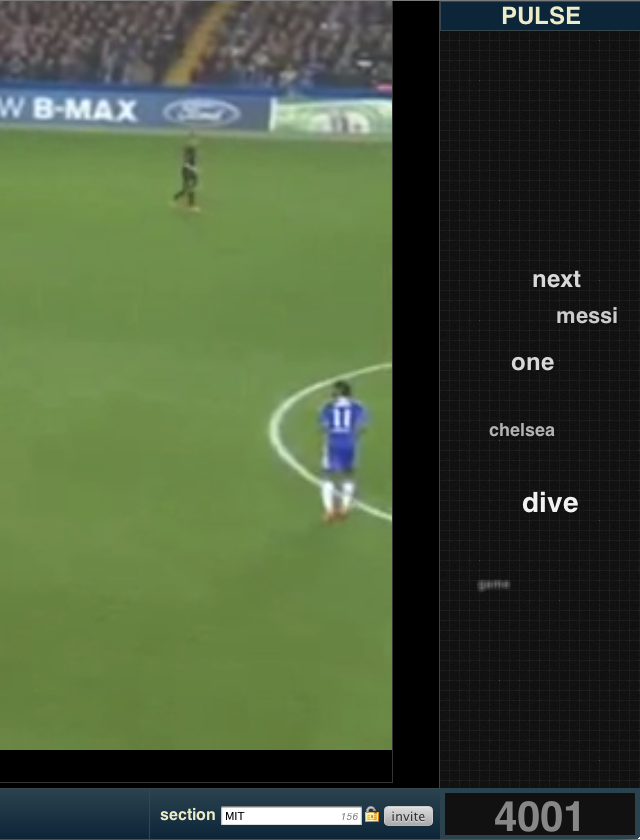
\includegraphics{figures/roar/bubble.png}
	\caption{Similar to the river-style visualization, in this approach words appear at the bottom and rise smoothly to the top. In this screenshot, there is relatively low activity.}
	\label{fig:pulse_bubble}
\end{marginfigure}

Returning back to the original values for this visualization, the final visualization approach meets all three goals in an acceptable (if not totally perfect) way. Volume is represented by the bursts of new words at the base of the visualization. This helps show instantaneous increases in participation. Furthermore, it has essentially the same property as the word-cloud approach where the total number of words on screen is loosely correlated with an average of recent activity. In this version, truly popular and long-lasting topics are better distinguished from transient topics, and new topics and easier to differentiate from popular old topics because of the way the words move through the visualization space. This also better supports the sorts of collective action concepts we have in mind; the words of a chant could appear out of the bottom one at a time and not be confused with prior words in the sequence. The biggest remaining weakness of this visualization is that its heavy reliance on motion could be distracting from the primary event content. To help alleviate this, the visualization could be easily run in a minimized mode where only one or two words at a time are shown and travel very slowly so as not to take away from the action during tense moments.

\begin{marginfigure}
	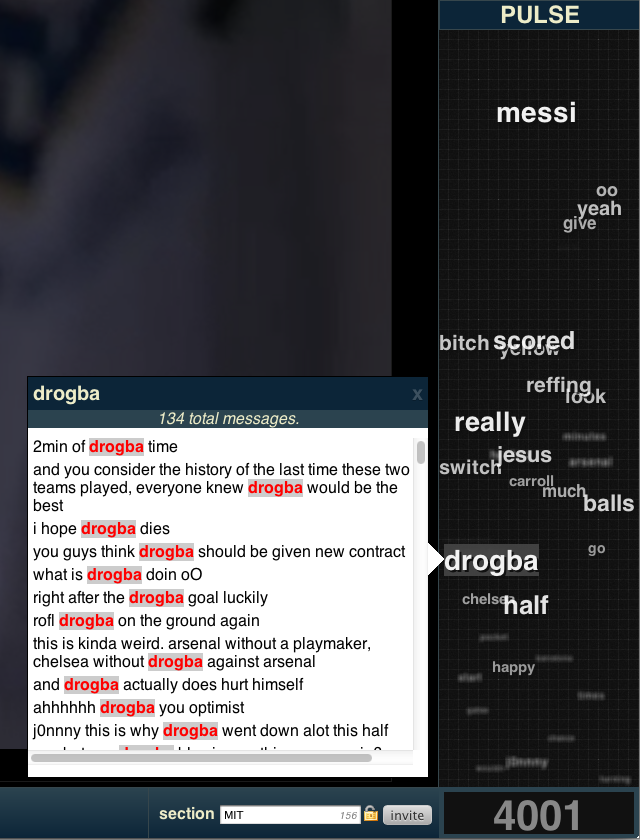
\includegraphics{figures/roar/bubble_detail.png}
	\caption{A view of the bubble-style visualization during a high activity period. Clicking on a term brings up a view of messages that led to that term's appearance in the term ranking list.}
	\label{fig:pulse_bubble_detail}
\end{marginfigure}


\subsection{Moderation}



% \section{Technology}
% write up the socket scaling stuff? seems silly in a design thesis with no other technology sections

